\documentclass[sigconf,review,anonymous]{acmart}

\usepackage{subcaption}
\usepackage{cleveref}

\crefname{figure}{Figure}{Figures}

\acmConference[SPLC'25]{29th International Systems and Software Product Line Conference}{September 01--September 05, 2025}{A Coruña, Spain}

\begin{document}

\title{Bridging Digital and Physical: Applying Software Product Line Engineering Principles to Digital LEGO}

\author{Aleksandra Erohina}
\affiliation{
    \institution{FH Upper Austria (FH OÖ)}
    \department{School of Engineering}
    \city{Wels}
    \state{Upper Austria}
    \country{Austria}
}

\author{Christian Zehetner}
\orcid{0000-0002-3149-8476}
\affiliation{
    \institution{FH Upper Austria (FH OÖ)}
    \department{School of Engineering}
    \city{Wels}
    \state{Upper Austria}
    \country{Austria}
}
\email{christian.zehetner@fh-ooe.at}

\author{Georg Hackenberg}
\orcid{0000-0003-3913-4148}
\affiliation{
    \institution{FH Upper Austria (FH OÖ)}
    \department{School of Engineering}
    \city{Wels}
    \state{Upper Austria}
    \country{Austria}
}
\email{georg.hackenberg@fh-ooe.at}

\begin{abstract}
    In this paper, we explore the application of software product line engineering (SPLE) principles to the development of physical products, specifically using digital LEGO as a case study. 
    By translating key concepts from the SPLE community, we demonstrate how modularity, variability management, and systematic reuse can enhance the design and production of physical products. 
    Our experience highlights the benefits and challenges of this interdisciplinary approach, providing valuable insights for both software engineers and product designers.
\end{abstract}

\keywords{Software Product Line Engineering (SPLE); Digital LEGO; Modularity; Variability Management; Systematic Reuse; Physical Product Design; Interdisciplinary Approach}

\maketitle

\section{Introduction}
\label{sec:introduction}

With today's shift from a seller's to a buyer's market, there is a clear trend towards product customization. 
Customers are constantly seeking products that cater to their specific needs and budgets. 
However, creating customer-specific designs can often be inefficient and costly, making it unaffordable for the average consumer.
Besides, in most industries very few or practically no systems are created “from scratch”, so engineers are likely to reuse knowledge from a previous project or product in the form of documents, processes, or models~\cite{Góngora_2015}. 

To find a balance between reuse and customization in software and systems development, software product line engineering (SPLE) has emerged as a viable solution. 
SPLE is an approach to cost-efficiently deriving tailored products for markets and customers, utilizing common components and services in a planned manner~\cite{Runeson_2012}.
The focus is shifted from building isolated products to building families of related products, while reuse is discussed not at an individual object level, e.g.~libraries or components, but as a whole: organizational, process-wise, and also lifecycle-wise end-to-end from requirements to actually deployed variability at the customer~\cite{Schwanninger_2009}. 
This approach involves the development of a core platform as well as reusable components that can be easily customized to meet the specific needs of different products within a product line. 

For example, software products that are being developed for the international market must be adapted for different legal or cultural environments, as well as for different languages, and so must provide adapted user interfaces~\cite{Beuche_2007}. 
To increase software reuse and streamline development processes, developers create a modular software framework that includes common functionalities. 
The framework modules then can be reused across different product models and customized as needed to meet specific requirements for each individual market and customer.

Originating in software development, SPLE principles have now spread far beyond the software domain. 
Companies in many other industries, such as automotive, aerospace, and consumer electronics are taking advantage of reusability and variability management while reducing time-to-market, improving efficiency, and increasing customer satisfaction. 
For instance, Lockheed Martin estimates that because of its SPLE-inspired approach it saves over \$47 million a year ~\cite{Gregg_2015}, while Hewlett-Packard reports that it builds products 10 times as complex, with 1/4 of the staff, in 1/3 of the time, and with 1/25 of the bugs of previous products ~\cite{Mebane_2007}.

However, when it comes to incorporating SPLE principles into the creation of technical systems, particularly when creating geometric representations of product lines of mechanical products, this approach has not yet become widely established. 

\paragraph{Research objective}

To overcome the current situation we work on translating established ideas and concepts from the software product line engineering community to the development of physical (and ultimately cyber-physical) products.
Also, we want to help improving and more widely establishing product line engineering education for designers of physical products.

\paragraph{Research question}

To reach our research objective, we tackle the following research questions here:
Can we use digital LEGO for building interesting use cases for product line engineering?
Can we see typical issues in product line engineering such as module (in-)compatibility in such use cases?
Can we use existing digital LEGO tools for building these use cases already today?

\paragraph{Contribution}

To answer these research questions, we first conduct a literature review on product line engineering in the software domain as well as other domains (see Section~\ref{sec:related-work}).
And then, based on the results of our literature review we derive a digital LEGO case study consisting of atomic modules, various configuration options, and a 150\% model (see Section~\ref{sec:case-study}).

\section{Related work}
\label{sec:related-work}

Subsequently, we first summarize the relevant state-of-the-art of product line engineering (PLE).
First, we describe common principles and methodologies in the field of PLE in Section~\ref{sec:principles}.
Then, we explain the concept of modules and non-contact as well as contact-based mechanical interfaces in Section~\ref{sec:modules}.
Finally, we explore the representation of the product line and its individual variants in Section~\ref{sec:variants}.

\subsection{Principles and methodologies}
\label{sec:principles}

A product line can be seen as a set of individual products that share a common, managed set of features addressing the specific needs of particular market segments or missions and that are derived from a common set of core assets in a systematic way~\cite{Clements_2002}.
In this context, a feature denotes a characteristic of a member product in a product line that distinguishes it from other member products in the product line~\cite{ISO/IEC_26550}.
Van der Linden et al.~\cite{Linden_2007} formulated several principles that are fundamental in PLE including, among others, the principle of the two-lifecycle approach, which comprises the domain engineering and the application engineering lifecycle, and the principle of variability management.

Domain engineering is a reuse-based approach defining the scope (i.e., domain definition), specifying the structure (i.e., domain architecture), and building the assets for a class of systems, subsystems, or member products~\cite{ISO/IEC_26550}.
During domain analysis, developers determine the scope of the product line and identify its common and variable features, which they then document in a variability model. 
A number of techniques have been developed to manage variability.
For our case study, we use the orthogonal variability model (OVM) introduced by Pohl et al.~\cite{Pohl_2005}, which uses variants and variation points to denote variability, and dependencies to define relationships between variants and variation points.

In contrast, application engineering represents the process of deriving a single product variant that is tailored to the requirements of a specific customer, based on the results of domain engineering~\cite{Kästner_2013}. 
Note that with the appearance of second-generation PLE, the importance of the application engineering process steadily decreases, while products are derived through the use of high-end industrial-strength automation that configures the shared assets appropriately for each product~\cite{Krueger_2013}.

\subsection{Modules and interfaces}
\label{sec:modules}

Next, it is worth mentioning that PLE goes hand in hand with the concept of modularity.
While modularity enables the configuration of multiple end products from a limited number of modules, PLE manages and optimizes a company's product diversity in order to control complexity and to balance out too many variants and versions.
Li et al.~\cite{Li_2019} explain modularity as a systematic approach where a product or system is composed of various modules, and these modules can be combined in different ways to form different products with individual characteristics.

However, clear rules should be defined to reassure that all subsystems will be compatible and function correctly in the final design~\cite{Baldwin_2003}.
Such rules concern, among other things, the syntactic and semantic module interfaces, which define how the modules can be connected and interact.
The effects of a misspecified interface can go beyond module incompatibility to unexpected product behavior~\cite{Parslov_2015}. 

When applying PLE principles to the development of physical products, it is important to consider the physical nature of module interfaces.
Ulrich ~\cite{Ulrich_1995} states, that interfaces may involve mechanical, contact-based interactions between components in addition to non-contact interactions.
Such contact-based interactions usually entail constraints on the contact points of the mechanical surfaces to guarantee the required function of the assembly.
By specifying these constraints in computer-aided design (CAD) models, designers can ensure the proper arrangement and compatibility of parts within the products of the product line.

\subsection{Variants and representations}
\label{sec:variants}

The digital representations of the individual products in a product line can include, but are not limited to, requirement and design specifications, system and computer-aided design (CAD) models, source code and build files, test plans and cases, user documentation, repair manuals and installation guides, project budgets, schedules and work plans, product calibration and configuration files, data models, parts lists, and more~\cite{Clements_2015}. 

A wide-spread technique for the digital representation of product lines and their product variants are so-called 150\% models~\cite{Clements_2015}.
Such models combine all relevant features and characteristics of all product variants of the product line into a common superset model.
Furthermore, such models include all possible configurations of features and characteristics for all the variants and, hence, provide a complete picture of the product line.

Such superset representations of products lines and their variants have been applied successfully not only to software systems, but also to cyber-physical production systems and their various interdisciplinary subsystems~\cite{Fadhlillah_2023}, digital twins of physical products with advanced simulation capabilities~\cite{Wagner_2024}, and assembly instructions for configurable physical products~\cite{Zogopoulos_2024}.

\section{Case study}
\label{sec:case-study}

In this third section we introduce the case study, which we prepared for testing the applicability of digital LEGO based on the open LDraw\footnote{\url{https://ldraw.org}} data format and parts library for product line engineering education in a physical product design context.
The selected product line includes three first person view (FPV) drone variants: an \textit{ultralight drone}, a \textit{freestyle drone} and a \textit{long-range drone}, which differ primarily in their performance characteristics.

\begin{figure*}[tbp]
    \subcaptionbox{Small propeller\label{fig:propellor-small}}{
        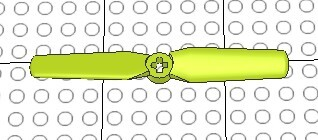
\includegraphics[height=1cm]{./drone-case-modules-propellor-2-small.jpg}
    }
    \hfill
    \subcaptionbox{Medium propeller\label{fig:propellor-medium}}{
        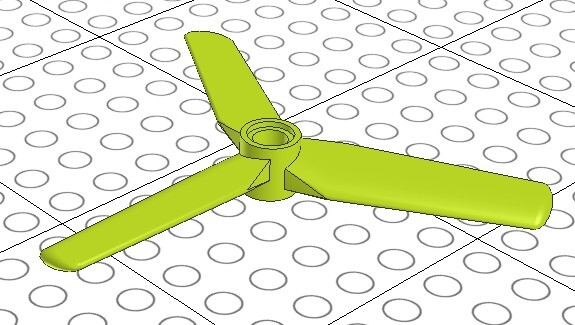
\includegraphics[height=1cm]{./drone-case-modules-propellor-3.jpg}
    }
    \hfill
    \subcaptionbox{Large propeller\label{fig:propellor-large}}{
        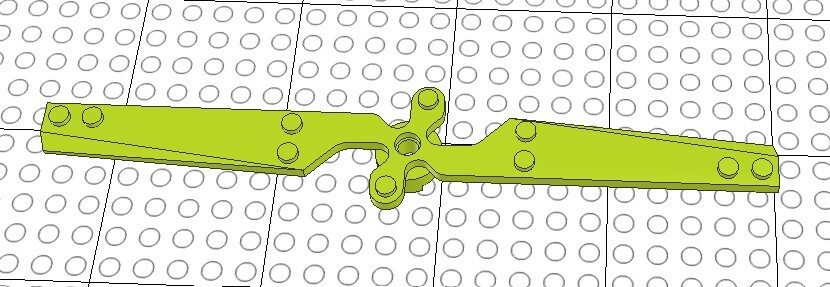
\includegraphics[height=1cm]{./drone-case-modules-propellor-2-large.jpg}
    }
    \hfill
    \subcaptionbox{Small battery\label{fig:battery-small}}{
        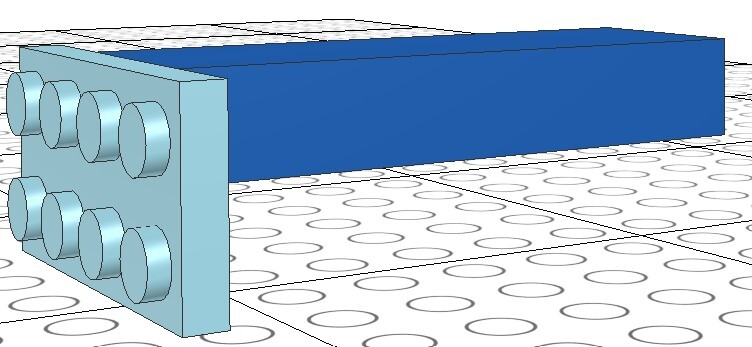
\includegraphics[height=1cm]{./drone-case-modules-battery-small.jpg}
    }
    \hfill
    \subcaptionbox{Medium battery\label{fig:battery-medium}}{
        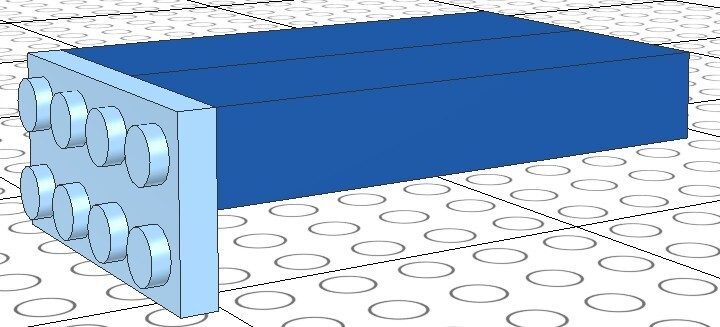
\includegraphics[height=1cm]{./drone-case-modules-battery-medium.jpg}
    }
    \hfill
    \subcaptionbox{Large battery\label{fig:battery-large}}{
        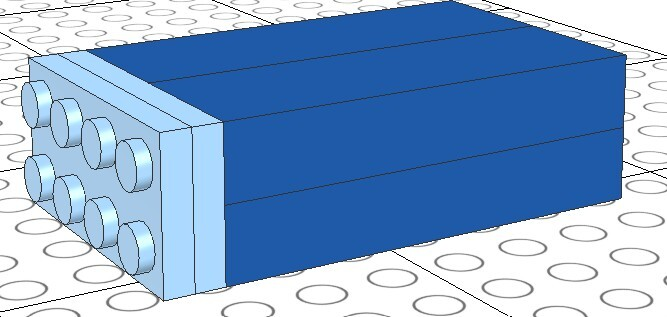
\includegraphics[height=1cm]{./drone-case-modules-battery-large.jpg}
    }

    
    \subcaptionbox{Small frame\label{fig:frame-small}}{
        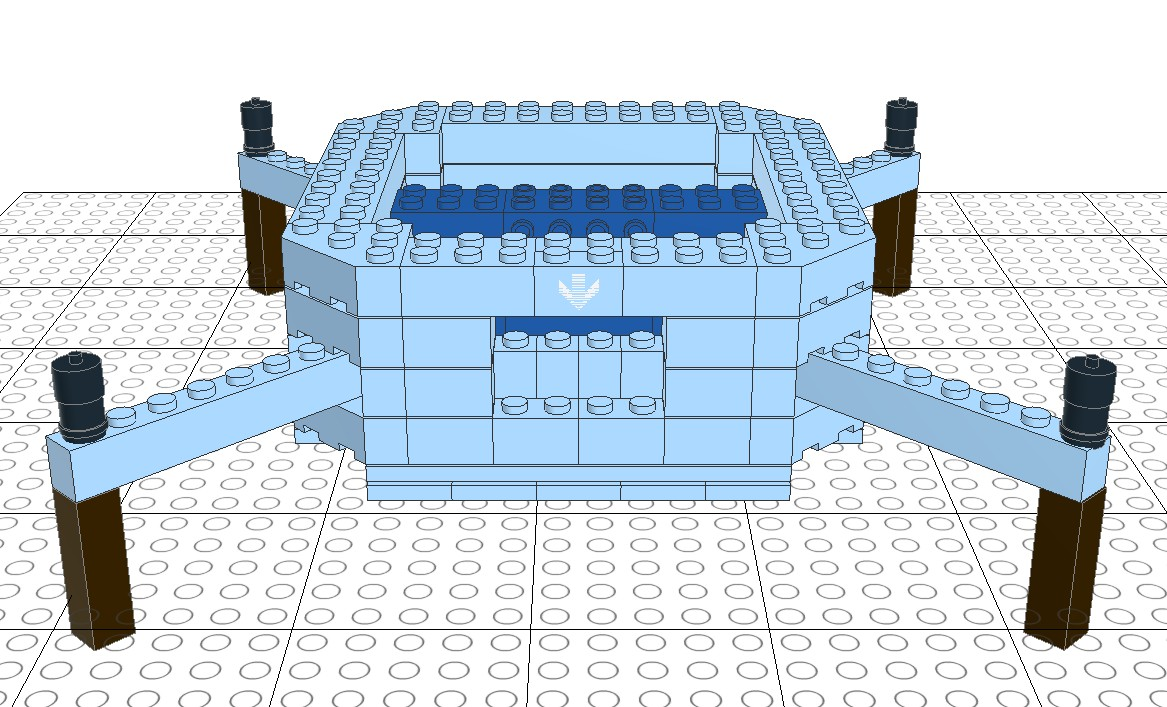
\includegraphics[height=2.1cm]{./SmallFrame.jpg}
    }
    \hfill
    \subcaptionbox{Large frame\label{fig:frame-large}}{
        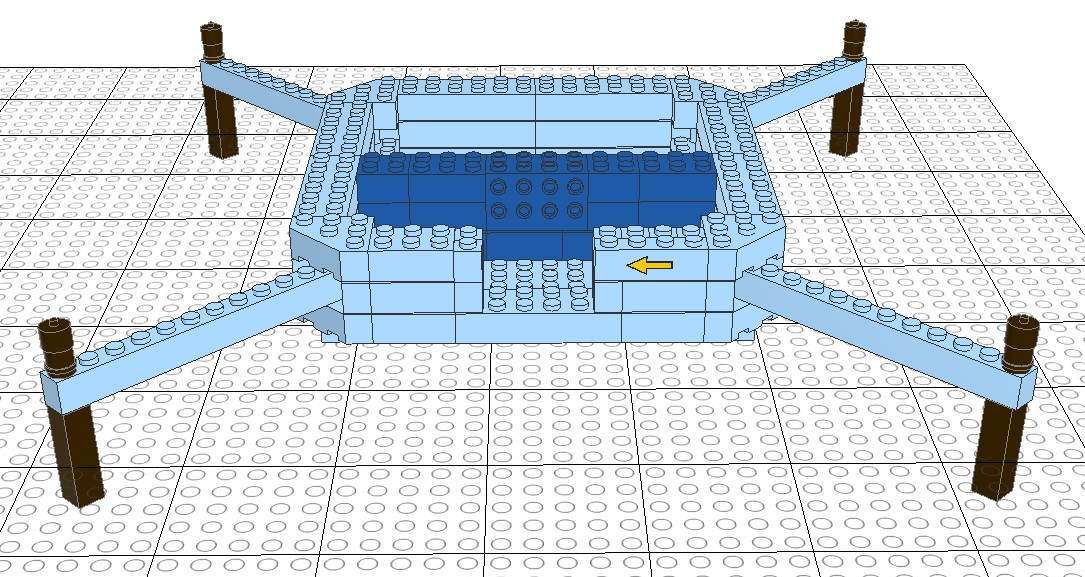
\includegraphics[height=2.1cm]{./LargeFrame.jpg}
    }
    \hfill
    \subcaptionbox{Small cover\label{fig:cover-small}}{
        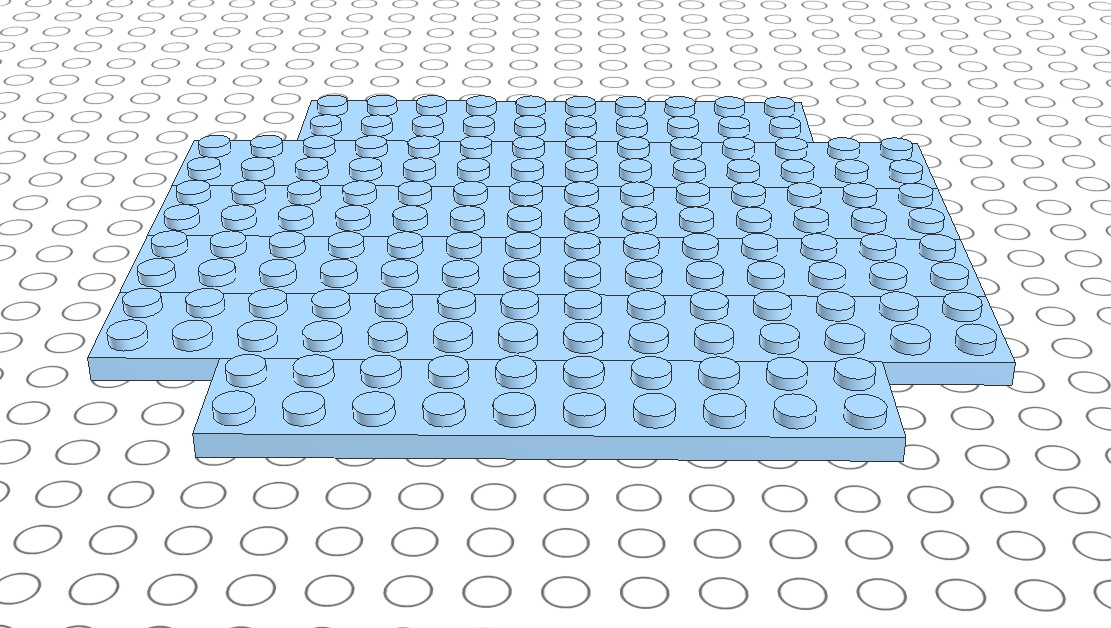
\includegraphics[height=2cm]{./SmallCover9.jpg}
    }
    \hfill
    \subcaptionbox{Large cover\label{fig:cover-large}}{
        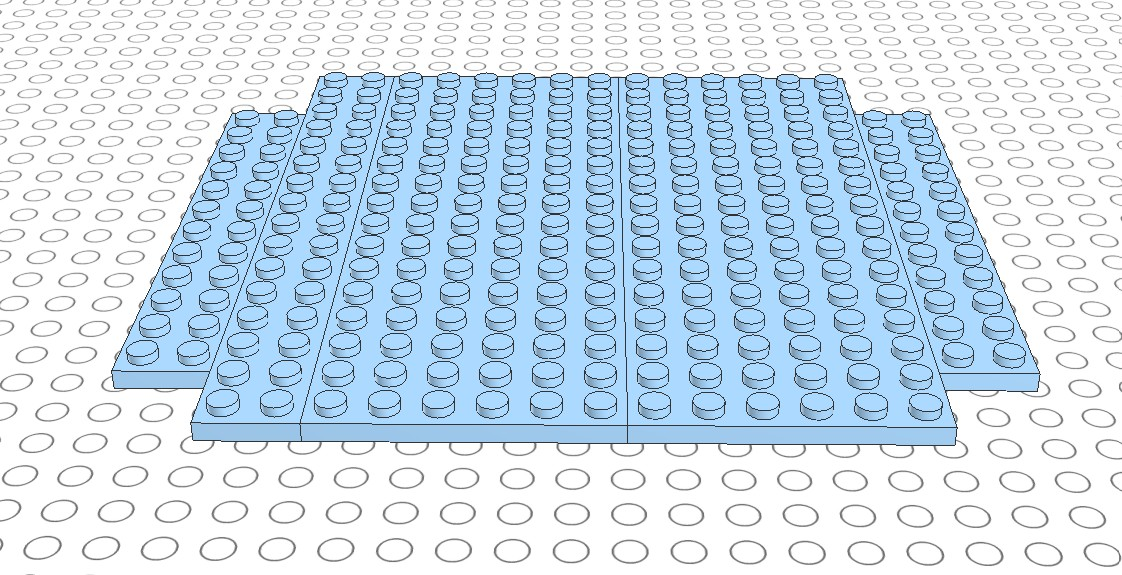
\includegraphics[height=2cm]{./LargeCover9.jpg}
    }

    \caption{Overview of the atomic (mechatronic) modules for the drone use case.}
    \label{fig:atomic-modules}
\end{figure*}

Subsequently, we first provide an overview of the atomic (mechatronic) modules of the product line, from which the individual variants can been assembled in Section~\ref{sec:atomic-modules}.
Then, we introduce a number of contact-based mechanical interface contraints governing the composition of the atomic modules in Section~\ref{sec:contraints}.
Thereafter, we explain the configuration options of the drone use case in the form of an orthogonal variability model (OVM) in Section~\ref{sec:configuration-options}.
And finally, we introduce the 150\% LDraw (or digital LEGO) model for the drone use case including all atomic modules as well as the assembly structures of the three different drone variants in Section~\ref{sec:150-model}.

\subsection{Atomic modules}
\label{sec:atomic-modules}

The atomic modules (see \cref{fig:atomic-modules}) include propellers, batteries, frames, and covers each adding required system functionality and coming in different sizes with different physical and performance characteristics.
In the following, we explain each class of atomic module as well as their functionality in the context of the drone use case and the available sizes in more detail.

\subsubsection*{Propellers}
\label{sec:propellers}

The propellers (see \cref{fig:propellor-small}, \cref{fig:propellor-medium}, and \cref{fig:propellor-large}) generate thrust by spinning rapidly, allowing a drone to move in all directions. 
The small and large two-blade propellers provide better efficiency and longer flight times, while the medium triblade propeller offers more stability and maneuverability. 
Also note that in general smaller propellers provide better agility, while bigger ones provide more thrust and efficiency, allowing the drone fly longer distances.
On the contrary, larger propellers also require more power to spin.

\subsubsection*{Batteries}
\label{sec:batteries}

The batteries (see \cref{fig:battery-small}, \cref{fig:battery-medium}, and \cref{fig:battery-large}) provide power for the drone to operate. 
The smaller capacity batteries are lighter and more compact, which can improve the agility and maneuverability of the drone. 
However, smaller batteries typically also have shorter flight times, which means that for longer flights a higher capacity battery is more suitable.

\subsubsection*{Frames}
\label{sec:frames}

The frames (see \cref{fig:frame-small} and \cref{fig:frame-large}) serve as the structure that holds all the other parts (legs and motors are pre-installed) together. 
The small frame is more maneuverable and agile, while a large frame offers more space for additional components (e.g.~larger batteries and possibly other equipment such as cameras and infrared sensors).

\subsubsection*{Covers}
\label{sec:covers}

The covers (see \cref{fig:cover-small} and \cref{fig:cover-large}) protect the internal components of the drone (i.e.~the batteries and other electronics), help to improve aerodynamics and serve an aesthetic purpose as well.
In alignment with the frames two cover sizes are provided, a small cover fitting the small frame, and a large cover fitting the large frame.

\subsection{Interface constraints}
\label{sec:contraints}

Physical interfaces between interacting modules enable their geometric connection. 
A frame for the drone example has three interfaces: with the batteries, with the propellers and with the covers. 
However, several geometrical constraints should be considered. These include:

\subsubsection*{Size and shape constraints}

Modules must be designed in such a way that they can physically fit together without interference. 
For the drone example, the large frame can accommodate all three types of batteries, while the small frame is limited to only small and medium batteries because of the size constraints.

\subsubsection*{Alignment constraints}

Modules must be aligned properly to ensure proper functioning when assembled together. 
For example, covers must be oriented correctly relative to frames to serve the protective and aesthetic purposes. 

\subsubsection*{Interference constraints}

It is important to consider potential interferences between modules, such as conflicting shapes or components that may impede proper assembly or operation. 
It is technically feasible to install any propeller on any frame, but practical constraints come into play. 
For instance, a large propeller cannot be mounted on a small frame without interference, as it would collide with the frame during rotation.
\cref{fig:feature-tree} illustrates constraint dependencies caused by these geometric restrictions.

\subsection{Configuration options}
\label{sec:configuration-options}

\begin{figure*}[htbp]
    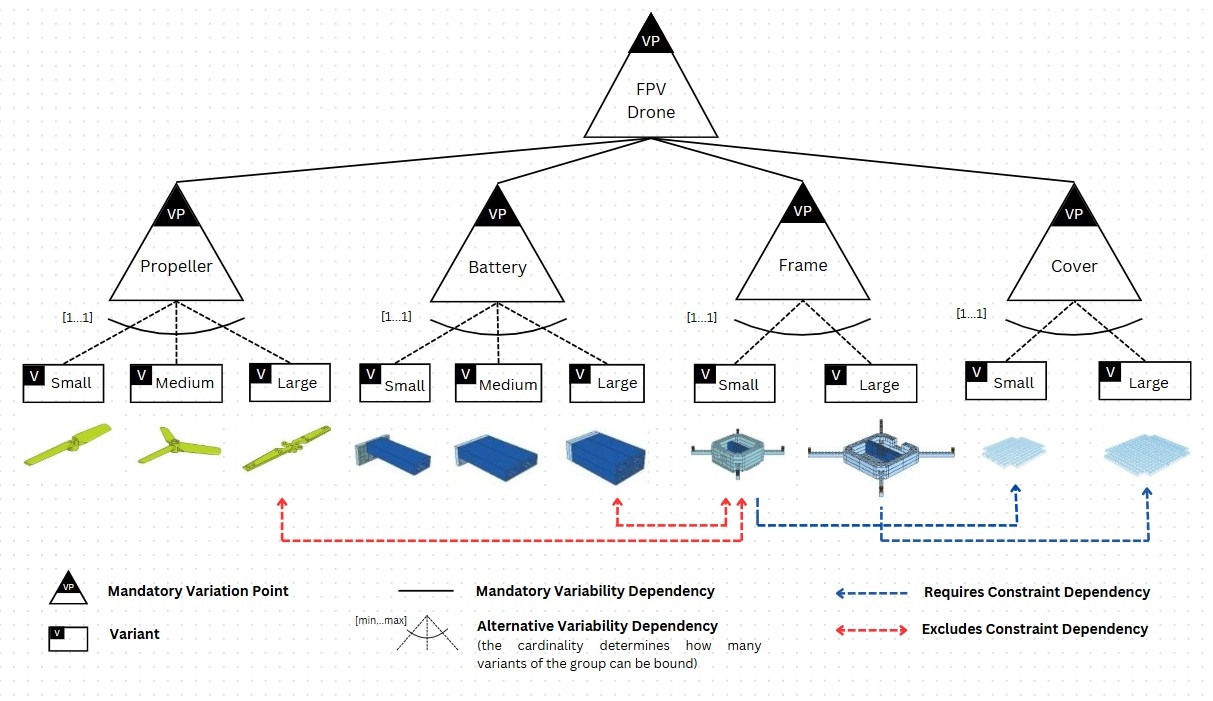
\includegraphics[width=\textwidth]{./FeatureTreeWithLegend3.jpg}
    \caption{Overview of the configuration options for the drone use case}
    \label{fig:feature-tree}
\end{figure*}

The modules can be combined to design customized end products.  
For that purpose, the FPV drone variability model is developed. 
When a customer wishes to design and buy a drone, multiple decisions have to be made before the final system can be build. 
\cref{fig:feature-tree} shows that the variation points Propeller, Battery, Frame and Cover have a mandatory dependency with the FPV drone, which means that they have to be included in the final product. 
For each of these variation points a variant has to be selected. 
The variants are connected by an alternative choice dependency with a minimum and maximum equal to one, which means that only one variant has to be chosen to be included to the final product. 
Additionally, two types of constraint dependencies exist: require constraint and exclude constraint. 
The require constraint means that when the small frame is selected, the small cover should be integrated to the system, and when the large frame is selected, the large cover should be integrated. 
The excluding constraint means that when a large propeller is selected, the small frame can not be integrated to the design and this relationship goes the other way round as well.

\subsection{Model representations}
\label{sec:150-model}

The case study demonstrates the utilization of digital LEGOs to create a 150\% model of a 3D drone architecture. 
The model is built in LeoCAD\footnote{Official LeoCAD website: \url{https://leocad.org}}, which, thanks to its intuitive user interface, is a useful tool for the teaching of various engineering concepts. 
LeoCAD adheres to the LDraw standard\footnote{Official LDraw website: \url{https:/ldraw.org}}. 
\cref{fig:ldraw-standard} demonstrates a meta-model of the LDraw file. The file contains multiple assemblies. 
Each assembly contains multiple references, which point to either a model (which itself can contain sub-assemblies) or bricks (which are standardized and belong to a brick catalog). 
The reference includes transformation data (position, orientation) and optional appearance data (color).

Within the structure of the LDraw file, a main model shown in \cref{fig:150-model} serves as the foundation where all three variants of the drone are instantiated. 
Each variant is further segmented into submodels, which consist of modular components. 
These modules are essentially instances of the submodels, all organized within the same file.
The main model serves as the primary assembly, the three different drone variants are also categorized as assemblies. 
Moreover, components such as modules (e.g., covers, frames, batteries, and propellers) are also classified as assemblies. 
An assembly consists of children, where each child is linked to either a brick or another assembly. 

%\begin{figure}[htbp]
%    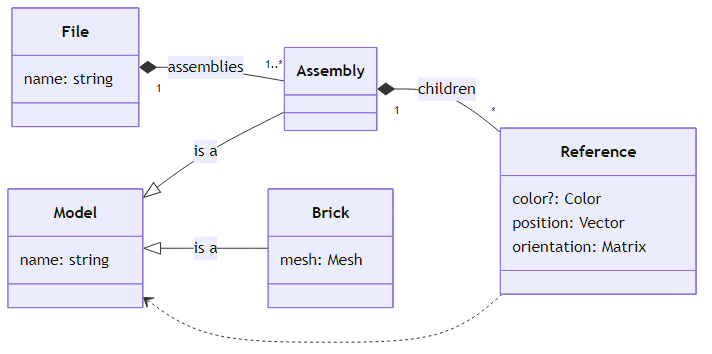
\includegraphics[width=\columnwidth]{./ldraw-standard.png}
%    \caption{LDraw standard}
%    \label{fig:ldraw-standard}
%\end{figure}

The approach enables to reuse the modules and submodels, promoting efficiency and versatility in design. 
The 150\% model encompasses all feasible combinations of drone features across the different variants. 
This abundance of information extends beyond the actual requirements of a specific drone type; for instance, showcasing three distinct battery sizes even though a practical FPV drone would only utilize one.

% \begin{figure}[htbp]
%     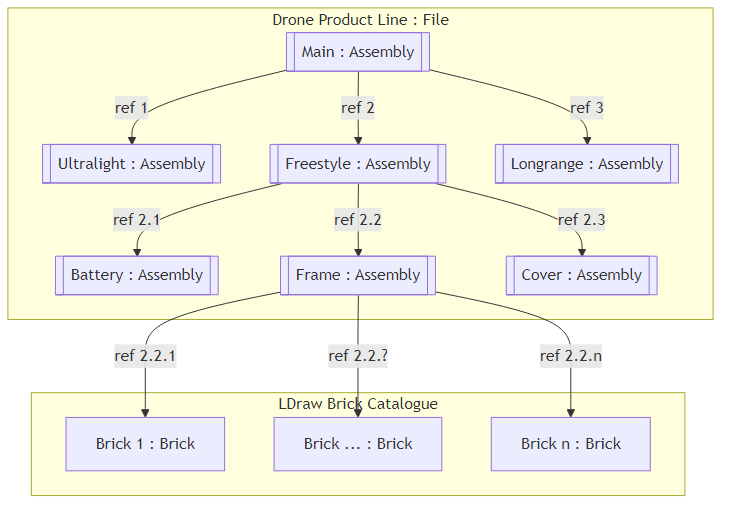
\includegraphics[width=\columnwidth]{./ldraw-model.png}
%     \caption{LDraw model}
%     \label{fig:ldraw-model}
% \end{figure}


\begin{figure*}[htbp]
    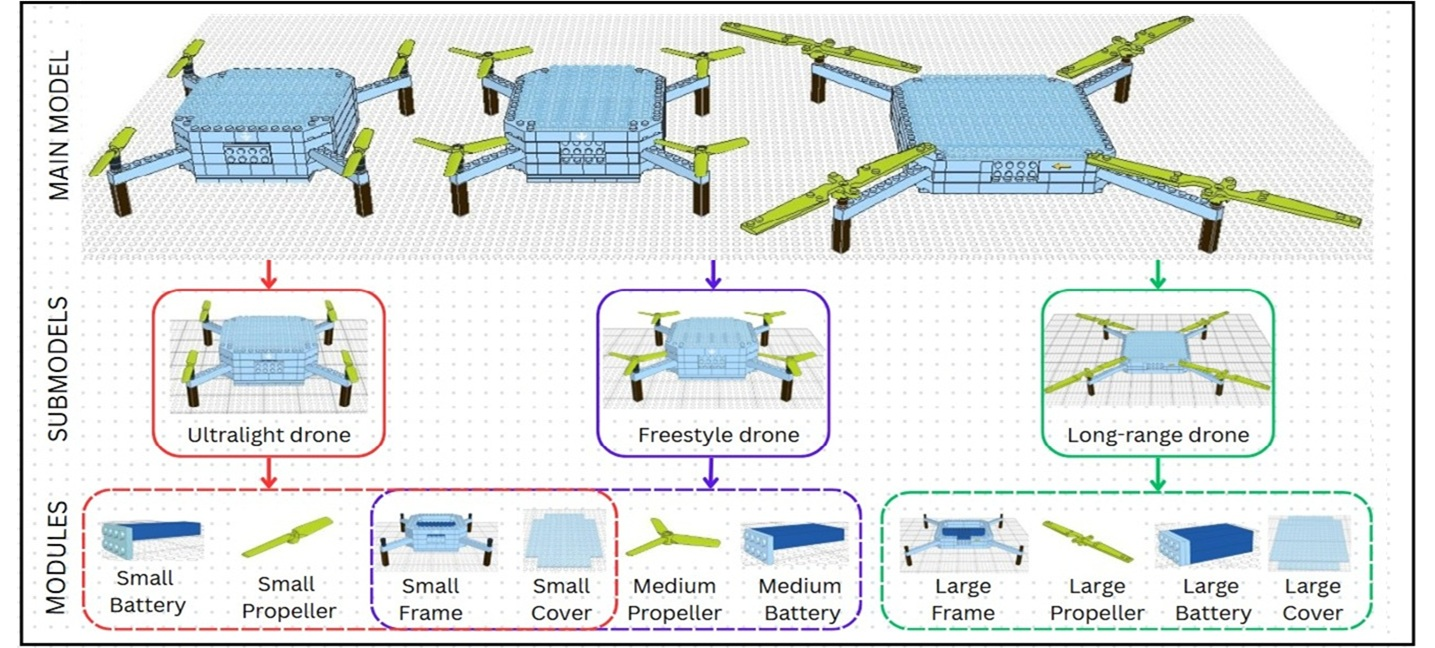
\includegraphics[width=\textwidth]{./150_MODEL_8.jpg}
    \caption{Overview of the 150\% model for the drone use case}
    \label{fig:150-model}
\end{figure*}

\section{Conclusion}
\label{sec:conclusion}

The knowledge acquired from the literature review coupled with the case study have provided a comprehensive demonstration of how SPLE principles can be effectively applied to the development of physical products with the usage of digital Lego. 
The first step was to create atomic drone modules, which could then be assembled into individual variants. 
Then, a robust variability model and a comprehensive 150\% model were developed. 
By utilizing these methodologies, we were able to derive a product line comprising three distinct drone variants from the model. 
This allowed us to demonstrate how well digital LEGO is suited to the 150\% modelling and reuse of modules across the entire product line.

In the next steps, we plan to explore geometric interfaces between components of physical products in a product line. Unlike software engineering, the realm of interfacing in this context remains relatively uncharted, making it an interesting area for exploration. 
One aspect to consider is the impact of a change to a single module on the entire product line. 
By examining whether such changes are consistent across all products in the line, we can gain insight into issues related to interface compatibility and mechanical stability. 
The use of digital LEGO is a very promising way to explore this area in an easy way.

\bibliography{main}
\bibliographystyle{ACM-Reference-Format}

\end{document}